\begin{figure}
	\begin{tikzpicture}
		\node at (0,0) {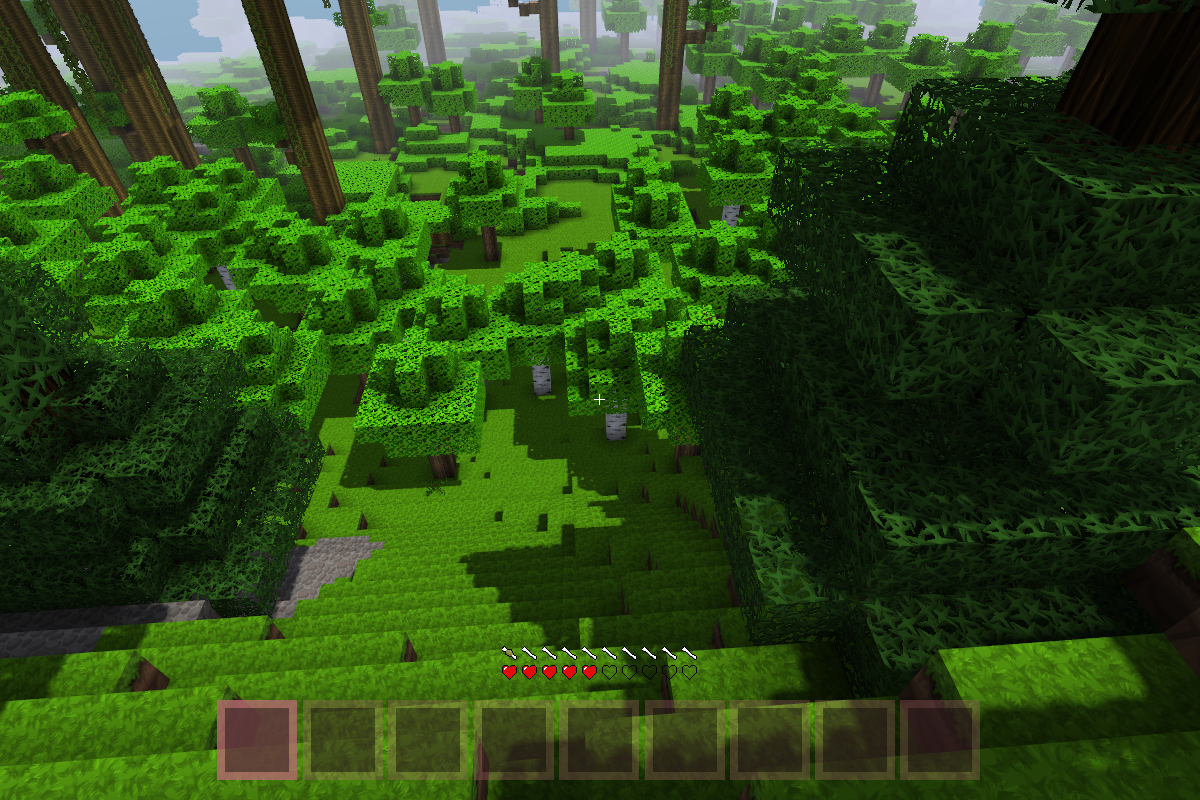
\includegraphics[width=.3\textwidth]{flackern-1.png}};
		\node[draw=red, circle, minimum size = 1.5cm] at (.25,-.5) {};
	\end{tikzpicture}
	\hfill
	\begin{tikzpicture}
		\node at (0,0) {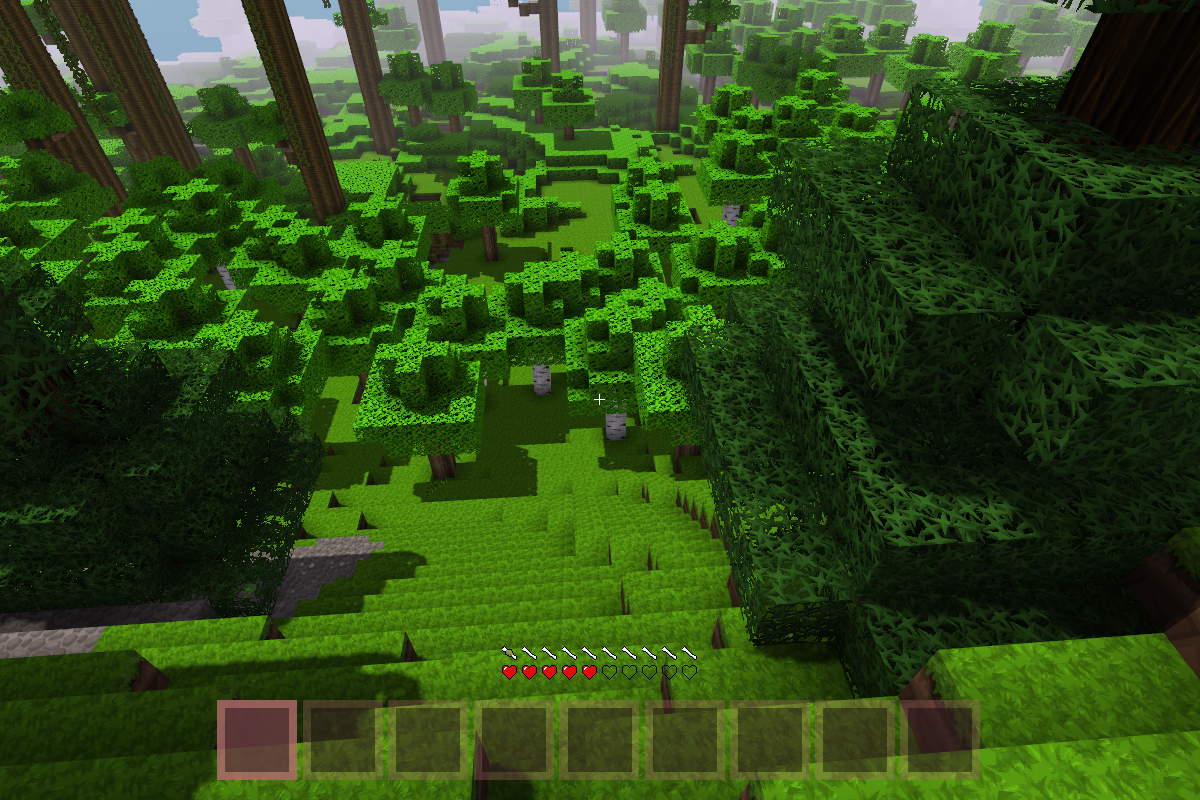
\includegraphics[width=.3\textwidth]{flackern-2.png}};
		\node[draw=red, circle, minimum size = 1.5cm] at (.25,-.5) {};
	\end{tikzpicture}
	\hfill
	\begin{tikzpicture}
		\node at (0,0) {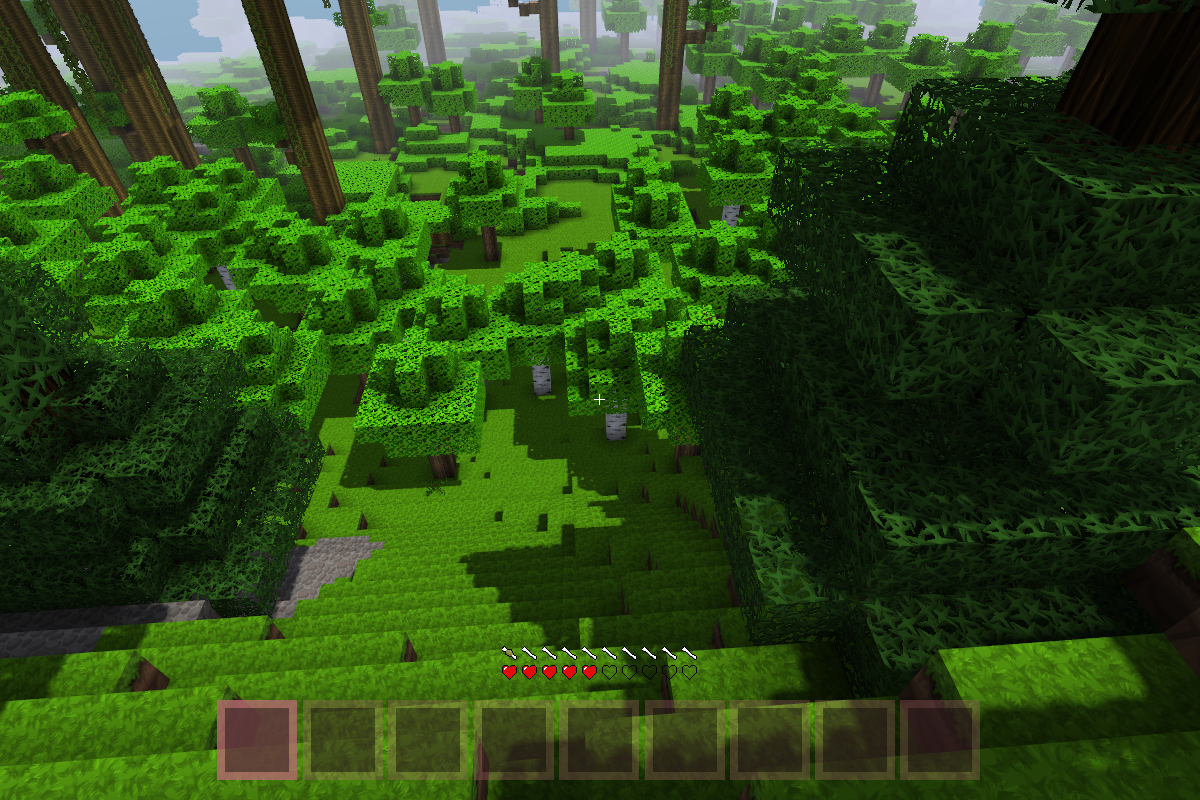
\includegraphics[width=.3\textwidth]{flackern-3.png}};
		\node[draw=red, circle, minimum size = 1.5cm] at (.25,-.5) {};
	\end{tikzpicture}
	\caption[Beispiel von flackerndem Schatten in der Blocklib.]{Beispiel von flackerndem Schatten in der Blocklib. Besonders der Schatten des rechten Baums (rot eingekreist) ist auffällig. Im Ablauf der drei Frames von links nach rechts ist er im mittleren Bild nicht zu sehen.}\label{fig:flackern}
\end{figure}
In diesem Abschnitt wird beispielhaft gezeigt, warum die Zwischenspeicherung des für das Rendering relevanten Spielzustands nötig ist. Dazu wird das Auftreten einer speziellen Wettkampfbedingung vor der Implementierung der Zwischenspeicherung beschrieben. 

Bei der parallelen Ausführung des Render-Threads ist bei der Darstellung der Schatten ein Flackern zu erkennen, das beispielhaft in Abbildung~\ref{fig:flackern} zu sehen ist. Die Tatsache, dass das Flackern in irregulären Intervallen auftritt, lässt auf das Vorhandensein einer Wettkampfbedingung schließen. Diese Vermutung kann dadurch bestätigt werden, dass das Flackern nicht mehr auftritt, sobald \code{update()} und \code{render()} sequentialisiert werden.

Da Variablen zeitgleich von verschiedenen Threads bearbeitet werden, ist die Suche nach dem Ursprung des Flackerns schwierig. Da der Fehler nur bei nebenläufiger Ausführung auftritt, müssen die problematischen Stellen auf \code{update()} und \code{render()} verteilt sein. Da der Fehler visuell sichtbar ist, lässt sich das Problem über die \glspl{Anweisung} in \code{render()} nachverfolgen. 

Eine naive Herangehensweise mittels Debugging ist nahezu unmöglich, da das Flackern unvorhersehbar auftritt. Zuerst muss also eine Möglichkeit gefunden werden, um das Auftreten des Flackerns programmatisch zu erkennen.

In der \classConfiguration{}-Klasse existiert die Variable \const{SHOW_SHADOW_MAP_FRAME}. Ist diese auf \code{true} gesetzt, wird in der linken oberen Ecke des Fensters ein Feld angezeigt, das die sogenannte \classShadowMap{} zeigt. Abbildung~\ref{fig:ShadowMap} zeigt einen Bildschirmfoto der Blocklib mit \code{SHOW_SHADOW_MAP_FRAME = true}. Die \classShadowMap{} wird genutzt, um zu berechnen, an welchen Stellen Schatten gerendert werden.
\begin{figure}
	\centering
	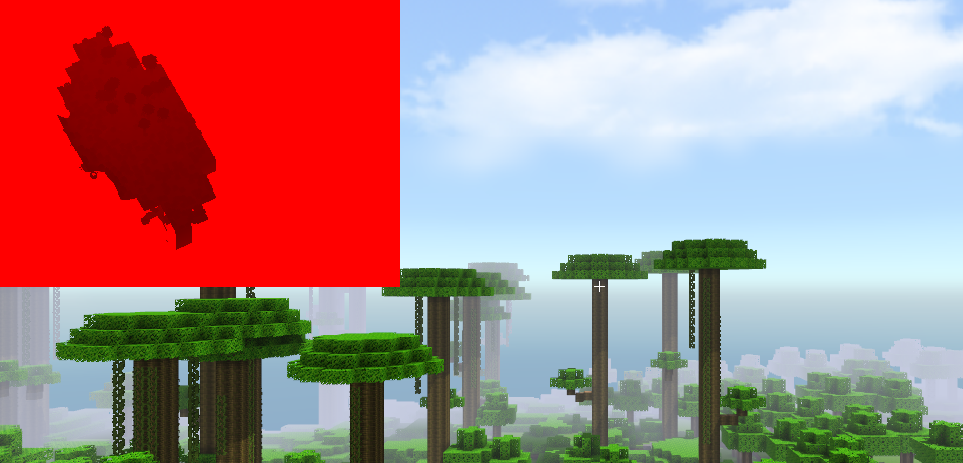
\includegraphics[width=.9\textwidth]{shadowMap.png}
	\caption[Ausschnitt eines Bildschirmfotos der Blocklib bei aktivierter \classShadowMap{}-Anzeige.]{Ausschnitt eines Bildschirmfotos der Blocklib bei aktivierter \classShadowMap{}-Anzeige. Die \classShadowMap{} speichert Entfernungs-Informationen, diese werden als rote Farbe interpretiert und ausgegeben, je größer die Entfernung, desto intensiver ist das Rot.}\label{fig:ShadowMap}
\end{figure}
\textcite{Ebbinger2018} beschreibt, wie das Rendering von Schatten in der Blocklib genau umgesetzt ist. Wie der Name der Klasse \classShadowMap{} vermuten lässt, wird für die Berechnung der Schatten das sogenannte \emph{Shadow-Mapping} verwendet. Dazu wird eine zweite Kamera implementiert, die die Spielwelt aus der Sicht einer Lichtquelle, im Fall der Blocklib der Sonne, betrachtet. Die so gerenderte Sicht wird dann genutzt, um zu berechnen ob ein Fragment, das heißt ein zu zeichnender Punkt auf dem Bildschirm, das erste Hindernis aus Sicht der Lichtquelle ist. Ist dies der Fall, so wird das Fragment beleuchtet, ansonsten ist etwas anderes vor dem Fragment und es befindet sich im Schatten.

Wird die \classShadowMap{} mit angezeigt, so kann man erkennen, dass diese sich zeitgleich mit dem Flackern verschiebt. Die Position der \classShadowMap{} wird über die Klasse \classShadowBounds{} bestimmt. Die Position muss in zwei Fällen geändert werden, zum einen, wenn die Sonne sich bewegt, also, wenn der Tag-Nacht-Zyklus aktiv ist, zum anderen, wenn sich die Spielerkamera bewegt, da das in der \classShadowMap{} gerenderte Bild immer der Position und dem Blickwinkel der Kamera angepasst werden muss.

Die Ausgabe der Position der \classShadowBounds{} während des Spiels bei deaktiviertem Tag-Nacht-Zyklus und stillstehender Spielerkamera bestätigt, dass diese Position sich tatsächlich zeitgleich mit dem Auftreten des Flackerns verändert. Das Auftreten der Wettkampfbedingung lässt sich also erkennen, indem eine Änderung der Position der \classShadowBounds{} in aufeinanderfolgenden Frames erkannt wird.

Nun gilt es die Ursache der Positionsänderung ausfindig zu machen. Die Position der \classShadowBounds{} hängt selbst von mehreren Variablen ab. Verfolgt man den Verlauf der Änderungen, finden sich die folgenden Abhängigkeiten:

\begin{tabular}{ll}
	\classShadowMap{} &$\to$ \code{ShadowBounds.update}\\
	& $\to$ \classLightViewMatrix{}\\
	& $\to$ \code{DayNightLighting.getSunUp()} \\
	& $\to$ \code{DayNightLighting.position}\\
	& $\to$ \code{DayNightLightig.updateLightPosition(...)}
\end{tabular}

\code{DayNightLightig.updateLightPosition(...)} wird nicht im Render-Thread ausgeführt, sondern während \code{update()} in einem anderen Thread. Der relevante Abschnitt der Methode ist in Listing~\ref{lst:raceLight} dargestellt.
\begin{lstlisting}[caption={Wettkampfbedingung in \code{updateLightPosition(...)}.},label={lst:raceLight},float={htbp}]
private void updateLightPosition(float progress, boolean day) {
	// ...
	position = new Vector3f(direction.x, direction.y, direction.z);
	position.scale(SUN_HEIGHT); (*\label{lst:updateLightPosition:scale}*)
	// let sun stay relative to the player
	position = Vector3f.add(position, Context.getInstance().getCamera().getPosition(), new Vector3f());
}
\end{lstlisting}
Wird also der Wert von \code{DayNightLighting.position} im Render-Thread ausgelesen, während die Methode in Ausführung ist, beispielsweise während Zeile~\ref{lst:updateLightPosition:scale}, so enthält \code{DayNightLighting.position} einen falschen Wert. Hier existiert also die gesuchte Wettkampfbedingung.

Diese Wettkampfbedingung ließe sich nun auch ohne eine Zwischenspeicherung des zu rendernden Spielzustands ansatzweise lösen, indem beispielsweise das Update der Position zu einer atomaren \gls{Anweisung} geändert wird. Um das zu implementieren, müsste das Attribut \var{position} als \code{volatile} deklariert werden. Dann kann die Berechnung der neuen Position auf einer temporären Variablen \var{newPosition} durchgeführt werden. Setzt man nun \code{position = newPosition} garantiert die Nutzung von \code{volatile} in Java, dass das Update atomar ist und sofort für alle anderen Threads sichtbar ist. Das Problem, dass nicht festgelegt ist, ob die Simulation vor der Nutzung der Variablen beendet ist, bleibt bestehen. Das führt jedoch lediglich zu Verzögerungen der Bewegung der Sonne um maximal einen Frame, was unbemerkbar ist.

Allerdings ist \var{position} nicht die einzige Variable, bei der es zu Wettkampfbedingungen kommt. Für jedes einzelne Modul müsste nachverfolgt werden, ob und wo es zu Wettkampfbedingungen kommen kann. Dann müsste an jeder Stelle individuell festgestellt werden, wie die Wettkampfbedingung zufriedenstellend beseitigt werden kann. Das ist ein zu großer Aufwand und birgt die Gefahr, dass Stellen übersehen werden. Daher ist die Zwischenspeicherung des zu rendernden Zustands notwendig.